\chapter{Implementation}
\label{implementation}

MCRP is implemented on the TelosB mote platform. It uses Contiki operating system as the software development (platform?) with full support of the standard IPv6. The implementation of MCRP are describe, including changes that were done (undertaken) in addition to the default parameters and settings for Contiki.

Contiki is a lightweight operating system with support for dynamic loading and replacement of individual programs and services. The purpose of the Contiki design is to reduce size and complexity, as well as to preserve flexibility. A running Contiki system consists of the kernel, libraries, the program loader and a set of processes (may be either an application program or a service - functionality used by more than one application process e.g. includes communication protocol stacks, sensor device drivers) \cite{contiki}. 
 
\section{Protocol Stack (changes at MAC, RT, NBR TB, BR etc.)}
MCRP is a cross layer protocol implemented on Contiki version 2.7. (explain what is cross layer? why do cross layer? FIGURE OF STACKS)

Contiki is a four layers network stack; network, MAC, radio duty cycling (RDC) and radio layers. The network layer includes support for TCP and UDP, IPv6, IPv4, 6lowpan and RPL (routing). Traditional TCP/IP implementations have required far too much resources which is impossible to fit in a sensor that has limited RAM capabilities (RAM is the most scarce resource). uIP \cite{uip} is a small RFC-compliant TCP/IP stack that makes it possible for Contiki to communicate over the Internet. uIP implementation is designed to have only the absolute minimal set of features needed for a full TCP/IP stack such as IP, ICMP, UDP and TCP protocols. The uIP is mostly concerned with the TCP and IP protocols and upper layer protocols \cite{contikiDoc, contikiUIP}. 

////BUFFER MANAGEMENT - since it's related to uIP (Chameleon, Rime etc)

\begin{table}
  \centering
    \begin{tabular}{|c|c|c|}
      \hline
      Contiki & IoT/IP & Applications \\
      \hline \hline
      \multirow{4}{*}{Network} 
        & Application & HTTP \\
        \cline{2-3}
        & Transport & TCP, UDP \\
        \cline{2-3}
        & Network, Routing & IPv6, IPv4, RPL \\
        \cline{2-3}
        & Adaptation & 6LoWPAN \\
      \hline \hline
      
      MAC & MAC & CSMA/CA \\
      \hline
      RDC & Duty Cycling & ContikiMAC \\
      \hline
      Radio & Radio & IEEE 802.15.4 \\
      \hline
    \end{tabular}
    \caption{Contiki Network Stack}
    \label{table:1}
\end{table}

It uses (EXPLAIN CONTIKIMAC - refer to contikimac paper; why it's good, how it works). Also about retransmission and buffers. (maybe at next section???) The transmitting channel is set at the MAC layer as packets are not send immediately if there are packets being queued. The channel is reset to the transmitting channel before it tries to send and it is then reset to the listening channel to wait and listen to any packets that is being sent to the node. 

The default ContikiMAC is a single channel protocol. It is modified to be able to work with multi channel nodes while (stick/hold/is) on the same principle of a low power ContikiMAC (minor changes to support multi channel without changing the main purpose of ContikiMAC).

RPL border router is used as LPBR in order to move most processing decisions on a PC as it has more RAM and better processing capabilities than a sensor. (Explain BR-SR how it works!)
TelosB has limited RAM and ROM of 10K bytes and 48K bytes of flash memory \cite{telosb-datasheet}. By using a border router, this allows channel changing to be decided in real time without draining the memory and battery on a sensor. The border router also acts as the root of the tree. The border router will setup the IPv6 prefix of the network and will initiate the creation of the RPL routing tree.
It (tunslip6) sets up an interface on the Linux IP stack and connects this interface via a socket to the border router node.
Border router is used to bridge the wireless IPv6 network to a PC via serial link which enables the IPv6 network traffic to reach outside network and the Internet.
A node is used as a wireless interface (IEEE 802.15.4 to enable the serial socket server), a host machine as border router to bridge the wireless IPv6 network to outside network and the Internet.

Serial Line Internet Protocol (SLIP) //need reference!!!] is used for the communication between the sink and the device which it connected to such as an embedded PC. SLIP is commonly used to encapsulate IP packets for transmission across the serial line of micro-controller devices. SLIP has a low complexity and small overhead. For the communication between the devices (embedded PCs), any reliable network can be used (e.g. Ethernet). The sinks are connected to an embedded PC which contains an Ethernet interface. The communication between the sink (sensor node) and the embedded PC makes use of SLIP. Contiki already provides support for SLIP communication and includes a tunslip tool (need reference!!!) which make it possible to communicate with devices using SLIP. The tool constructs a SLIP tunnel between a physical serial interface and a virtual network adaptor. By using tunslip the communication between the sink and the embedded PC is facilitated \cite{multipleSinks}.

Tunslip is a too used to bridge IP traffic between a host and another network element, typically a border router, over a serial line. Tunslip creates a virtual network interface (tun) on the host side and uses SLIP (serial line internet protocol) to encapsulate and pass IP traffic to and from the other side of the serial line. The network element sitting on the other side of the line does a similar job with it's network interface. The tun interface can be used like any real network interface: routing, traffic forwarding etc \cite{tunslip}.

RPL is used as the routing protocol. (explain how RPL works briefly since it's explained in LITERATURE REVIEW).

We tailored RPL control messages to be able to accommodate MRCP proposal by enabling unicast to know neighbours and broadcast to detect new nodes to join the tree.  


\section{MCRP Implementation}
MCRP is implemented as an extension to the existing implementation of RPL with ContikiMAC; to enable multi channel.
The protocol is implemented by tailoring existing code of ContikiMAC, network layer and RPL.

%\subsection{Application Layer}
//separate into 2; setCh and xSetCh as LPBR is separated with BR and SR
//access Network layer - Neighbour table, set channel

\subsection{Low Power Border Router}
As sensors have limited memory, we decided to move most decision making (processing decisions) at LPBR to a PC as it more RAM and better processing capabilities. This enables us to have more thorough processes. As describes previously, the protocol stack is divided into two main parts as shown is figure \ref{fig_lpbr} where the PC is responsible as the application, transport, network and routing layers while a sensor is set as the wireless interface to enable the PC to communicate with the other nodes. LPBR is a special case as channel changes at LPBR is not as direct as other sensor nodes due to this two parts. However, it works similar ways to the other nodes.

\begin{figure}
\centering
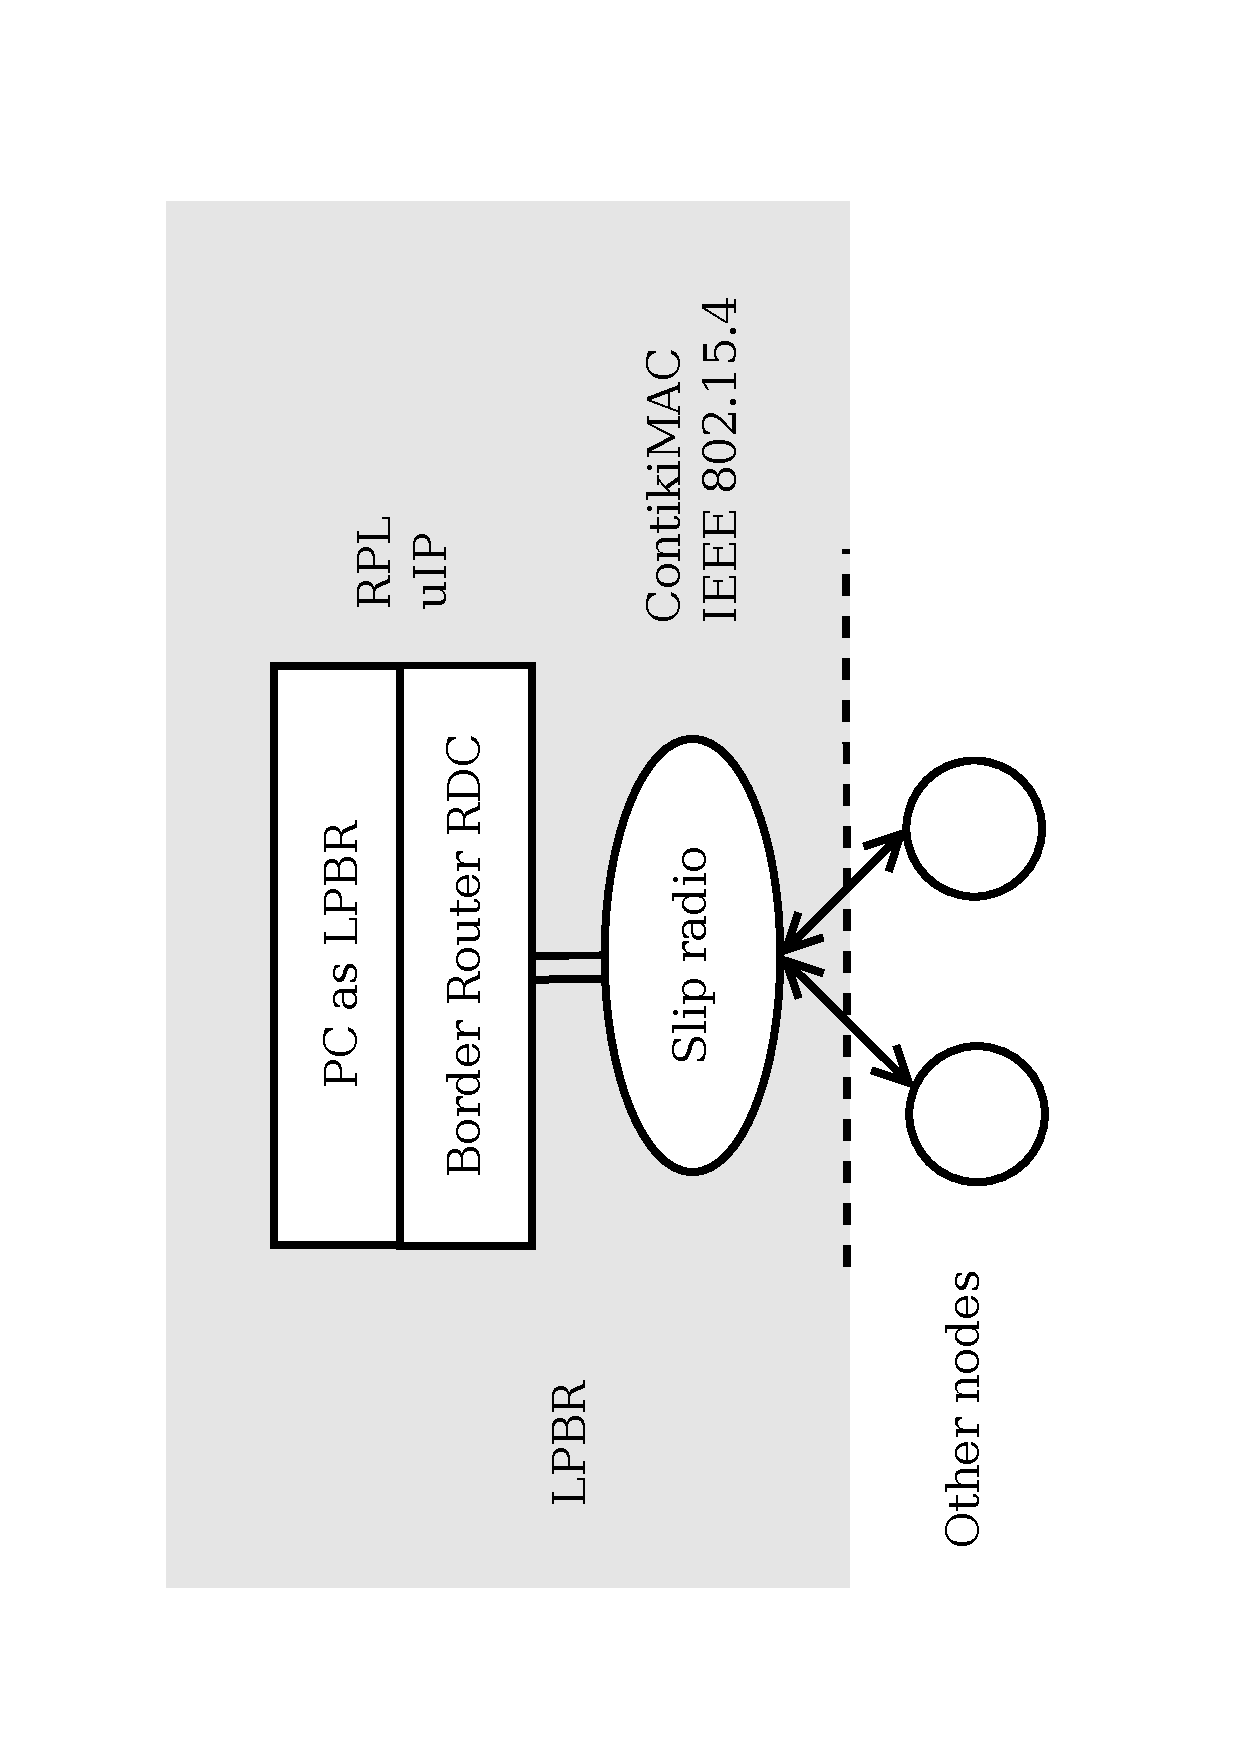
\includegraphics[trim=2cm 2cm 3cm 2cm, clip=true, totalheight=0.45\textheight, angle=270]{BR2.pdf}
\caption{Low power border router}
\label{fig_lpbr}
\end{figure}

%trim top left

LPBR main responsibility is to decide on the new channel selection. LPBR has no knowledge of all the channels condition at this point, thus, a channel is selected at random. LPBR keeps the results from the channel changes processes and based on it when selecting a new channel for the next node to ensure the new channel is at least two-hop away from another node using the same channel. This is done to ensure that the nearby nodes do not communicate of the same channel and risk interfering with each other.

The pseudo-code of the two-hops colouring algorithm that we implemented in new channel selection is shown in Algorithm \ref{twohop_algo}. When the new channel is selected, LPBR will send the value to the intended node.

\begin{algorithm}
\caption{Pseudo-code for two-hop colouring algorithm}
\label{twohop_algo}
\begin{algorithmic}[]
\\\textbf{Notations}
\\$R$ is a node that is a Route
\\$N$ is a node Neighbour
\\$RN$ is the Route's Neighbour node
\\$currentCh$ is the node current listening channel
\\$newCh$ is the new channel the node will change to
%\\$rnCh$ is the route's neighbour channel
\\\textbf{Pseudo-code}
%\If{$R$ $=$ $R$ in $LPBR$ $nodesTable$}
%	\State check $R$ $currentCh$
	\If{$R$ $currentCh$ $\neq$ $newCh$}
		\State succeed one-hop
		\State check all $RN$ channels
		\If{$RN$ channel $\neq$ $newCh$}
			\State succeed two-hop
			\State confirm $newCh$
		\EndIf
	\Else
		\State generate a new $newCh$
		\State update the number of $newCh$ generated for $R$
		\State use default channel 26 is all tries fail
	\EndIf
%\EndIf
\end{algorithmic}
\end{algorithm}

All layers of the netstack operate on the packet buffer. One buffer holds a single packet. ***Uses a single buffer for both incoming and outgoing packets \cite{uip, rime, rimeposter, contiki}. The packet buffer only holds the current packet.

Before passing to slip-radio, the header from $uip\_buf$ is compress to $packetbuf$.  
\cite{rime} introduces Chameleon, a communication architecture for sensor networks consists of Rime communication stack and a set of packet transformation modules. Rime communication stack provides a set of lightweight communication primitives ranging from best-effort anonymous local area broadcast to reliable network flooding. Protocols or applications running on top of Rime stack can implement additional protocols that are not in the Rime stack such as TCP/IP.

Rime draws heavily from communication abstractions for distributed programming where layers of simple abstractions are combined to form powerful high-level abstraction. The purpose of Rime is to simplify implementation of sensor network protocols and facilitate code reuse. The thin layers in Rime enable code reuse within the stack. An underlying MAC or link layer may chose to implement parts of the Rime stack \cite{rimeposter}.

Chameleon is a header construction. The parsing is done separately from the communication stack which allows the use of uIP or Rime communication stack that both are supported in Contiki.

6LoWPAN working group specified header compression and fragmentation for IPv6 over IEEE 802.15.4 (///REFERENCE!!!) and the IETF RoLL working group designed the RPL protocol as a proposed standard for IPv6 routing in low-power and lossy networks (LLNs). Contiki implement the necessary parts of the IPv6 protocol, IPv6 header compression and fragmentation with the 6LoWPAN adaptation layer, routing over LLNs with the RPL protocol, as well as a set of protocols from the TCP/IP protocol suite \cite{beyondInteroperability}.

Application can use either, both or none communication stack. uIP can run over Rime. Rime can run over uIP \cite{contikitutorial}. 

Buffer for uIP and Rime is the same. They use the same buffer.
 
Chameleon does not define any packet headers but instead uses $packet attributes$, an abstract representation of the information usually found in packet headers to allow applications to access low-level information without violating the layering principle. Packet headers are produced by separate header transformation modules that transform application data and packet attributes into packets with header and payload. The use of packet attributes makes it possible to adapt the output from the protocol stack to other communication protocols such as link and MAC layer protocols and TCP/IP.
Chameleon architecture allows for sensor network protocols that are implemented on top of the architecture to take advantage of the features of underlying MAC and link layer protocols.

In the buffer management of Chameleon architecture, all packets both outgoing and incoming are stored in a single buffer \cite{rimeposter}, called the Rime buffer. The Rime buffer contains both the application data and the packet attributes. All access to the Rime buffer is done at a single priority level so no locking mechanisms need to be used.

Protocols that need to queue packets, such as MAC protocols that wait for the radio medium to be free, can allocate so-called queue buffers to hold the queued packet. Queue buffers are dynamically allocated from a pool of queue buffers. The contents of the Rime buffer, including the packet attributes, are copied into the queue buffer when it is allocated.

The new channel is stored in the buffer before the data is sent over SLIP to the radio-chip (slip-radio). As the slip radio is unable to access the neighbour table where the next hop node channel is stored, the channel value is passed through the buffer. LPBR keeps the updated value of all it's neighbours channels in the neighbour channel. Slip radio that receives the packet buffer can access the channel value and kept the value is a simplified version of the neighbour table. This is done in order to ensure that the packet that is being queued or retransmitted are send on the correct channel. The packets destination, which in this case, the next hop node is first check before the packet is transmitted each time. The MAC layer sets the channel accordingly before sending. ContikiMAC can access the simplified neighbour table as it is on the slip radio. The simplified neighbour table only keeps the information of the node neighbours and neighbours channels which are the critical information in order to transmit packets correctly. The other information that is related to the neighbours conditions are monitored at the PC. 

\begin{figure}
\centering
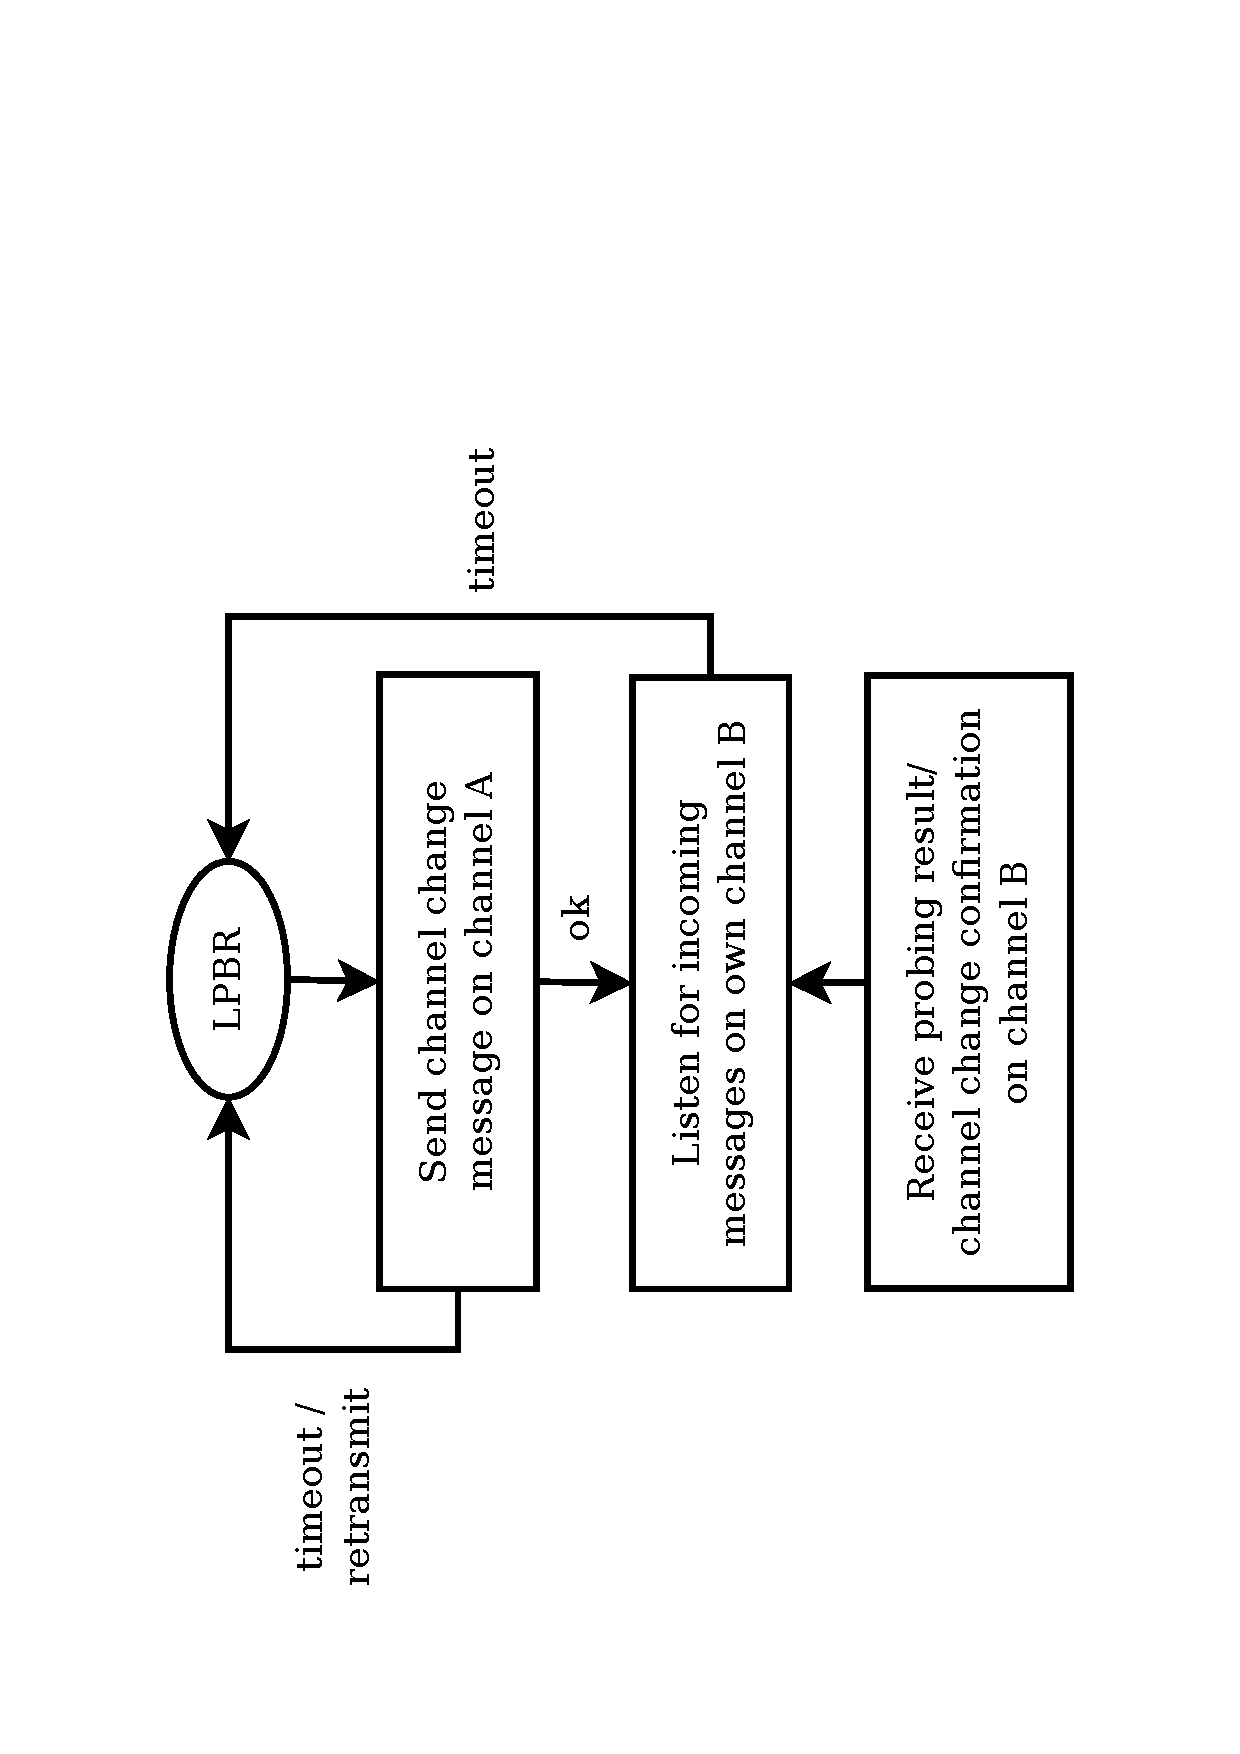
\includegraphics[trim=2cm 1cm 2cm 4cm, clip=true, totalheight=0.55\textheight, angle=270]{lpbrProcess.pdf}
\caption{LPBR processes}
\label{lpbrProcess}
\end{figure}
%top, left, bottom, right

LPBR processes are shown in \ref{lpbrProcess}.
The slip-radio resets to it's listening channel after the packet is transmitted. LPBR will wait and listen to any incoming packets. *In the channel probing phase, LPBR does not take part in probing. However, LPBR is informed of the results of probing and kept a table of the probing results and channels to be able to use the information when deciding on a channel change based on the previous results of probing on the known channels.

-send to BR RDC, check nbr table for the currentCh. pass the value to s-r. save the chvalue in a simplified nbr table to allow retx/queue to send on correct ch.
MAC set the channel accordingly before sending.
Change to its listening channel after finish sending. 

\subsection{Other Nodes (MAC Layer?)}
As MCRP is a cross-layer protocol, packets that have not been transmitted are kept in the buffer. In order for the transmission to be on the correct channel, the neighbour table in the network layer is accessed and the channel is set to the transmitting channel. 

ContikiMAC has retransmitted, collisions valued. These values are used in probing to decide on the channel condition. These values are passed to the application layer to decide on channel change. The packet can be retransmitted for ( ) times before it is dropped. However, if the channel is busy, and the packet has not been sent (collisions before sending), it can stay in the loop for a long time.

All nodes keep the neighbours channel in the neighbour table. Unlike LPBR, other nodes have all the layers within the node. This makes change changes less complicated, however, the nodes are being limited by the number of RAM is has which resulted in results of probing to be kept by the centralised LPBR. The node however, keep probing results temporarily before deciding on the channel. The node is cross-layer as it can access information at any layer.

When LPBR sends a channel change message to the destination node, the destination node will send a packet to acknowledge the channel change message. If LPBR does not receive the message, the channel change message is retransmitted. LPBR is then wait and listens for any incoming packets. At this point, channel changes processes will take place between the node and its neighbours.

The node sends the new channel to all the neighbours. At this point, the new channel is not check. However, all neighbours need to know the new channel as the node will be listening on the new channel. Otherwise, packets cannot be received by the node. The neighbours that receive the node channel will update their neighbour table at the application layer. As this is an important step in order to reduce the number of packet loss due to sending on the wrong channel, neighbours will send an acknowledgement of the new channel. Otherwise, it will be retransmitted. 

The node will then send a message to the neighbour that is a route node to start sending probing messages on the new channel. Not all neighbours are used routes. The neighbours are chosen as route based on RPL (//describe RPL briefly how if choose route). The node will listens on the new channel and wait for the probe message. The route node starts sending probing messages every 3 seconds to allow retransmission or collision that could happen due to the channel being busy (////what is retransmission? what is collision??? how it happens? how long? collision has no time out!). As the we are sending a small number of probing, to increase the channel reliability of the probing, we also take into account the number of retransmission and collision that happen. As the retransmission and collision is a link layer process, the values are kept in a table and is sent in the next probe message. This is because the value is only valid for that run. It gets reset each time a new packet is sent or received. The table is accessed at the application layer before the next probing message is sent. The probing message includes the number of tries the previous packet had taken before it is received. These values are used to decide if the channel is better than the current channel by giving a good probing result, meaning less retransmission.

The node keeps the value of probing messages it receives. It sends all the probing results to LPBR. LPBR could use the information to decide on a channel or blacklist bad channels. It then use the values to decide whether the new channel is better than the previous channel by setting a threshold. The node then send the channel that it confirms to be listening on to all neighbours. The channel can be the new channel or reverting to the previous channel. The neighbours will send an acknowledgement back to the node. This is also important to ensure that all neighbours could communicate with the node on the correct channel. The neighbours will update their neighbour table of the node channel. 


\subsection{Routing Layer - Neighbour Discovery}
///net/rpl/rpl-icmp6.c and rpl-timers.c - the changes done!!

////DIO UNICAST
RPL sends the control messages as broadcast. However, as we are now dealing with multi channels, using broadcast for all channels would waste the bandwidth and costly as it would take a longer time to go through all channels. It would also cause congestion and the node to be on the broadcast channel and not ready on it's listening channel to be able to receive any incoming packets as it has not finish with the control message broadcast. RPL DIO message is able to deal with either broadcast or unicast. By default, broadcast was used as RPL is usually used with a single channel MAC. We enable the unicast DIO.

////MULTI CHANNEL DIS
If a new node tries to join the tree, it will send a DIS message on all channels until it finds the neighbours. 

\section{Memory Footprint/Setup Overhead?}
-how many packets more than usual?
-memory consumption?